\documentclass[tikz, border=15pt]{standalone}
\usepackage{tikz}
\usetikzlibrary{calc}

\definecolor{nightsky}{HTML}{0B132B}
\definecolor{deepsky}{HTML}{1C2541}
\definecolor{goldfire}{HTML}{FFD166}
\definecolor{pinkfire}{HTML}{EF476F}
\definecolor{bluefire}{HTML}{118AB2}
\definecolor{lanternred}{HTML}{E63946}
\definecolor{lanternglow}{HTML}{FFB703}
\definecolor{stallwood}{HTML}{4A2810}
\definecolor{personcolor}{HTML}{080E1E}

\begin{document}
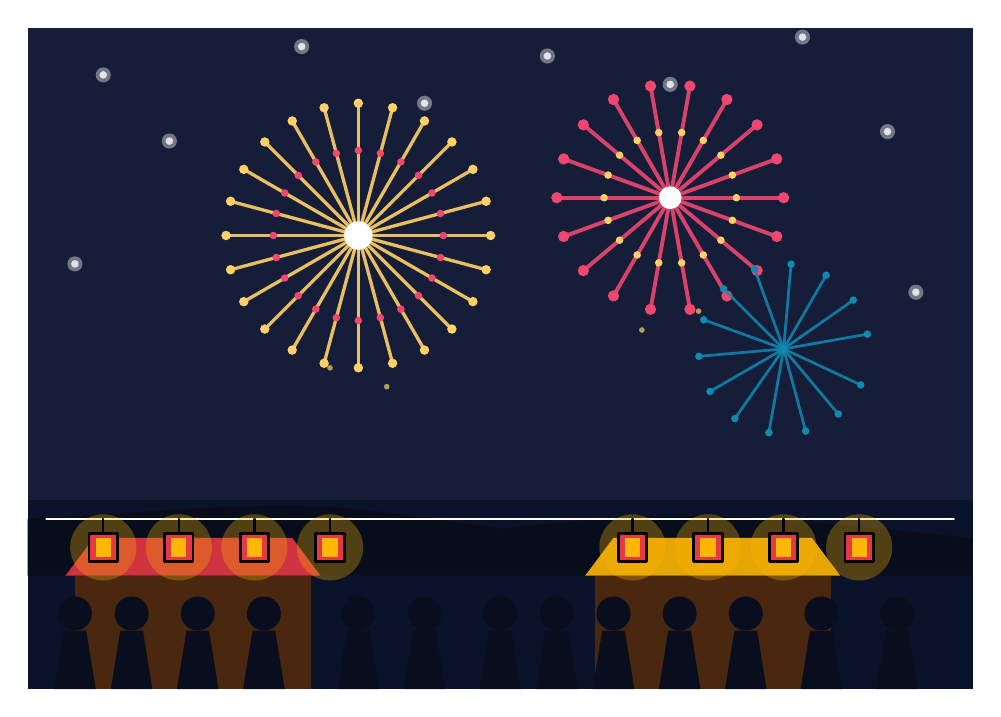
\begin{tikzpicture}[
    scale=1.2,
    line width=1pt,
    line join=round,
    line cap=round
]

    % Night Sky Background with Gradient Effect
    \fill[nightsky] (-5, -3) rectangle (5, 4);
    \fill[deepsky, opacity=0.6] (-5, -1) rectangle (5, 4);

    % Stars in Night Sky
    \foreach \x/\y in {-4.2/3.5, -3.5/2.8, -2.1/3.8, -0.8/3.2, 0.5/3.7, 1.8/3.4, 3.2/3.9, 4.1/2.9, -4.5/1.5, 4.4/1.2} {
        \fill[white, opacity=0.8] (\x, \y) circle (0.04);
        \fill[white, opacity=0.4] (\x, \y) circle (0.08);
    }

    % Fireworks 1: Main Gold & Red Burst (Center-Left: x=-1.5, y=1.8)
    \coordinate (FW1) at (-1.5, 1.8);
    \foreach \angle in {0, 15, ..., 345} {
        \draw[goldfire, line width=1.2pt, opacity=0.9] (FW1) -- ++(\angle:1.4);
        \fill[goldfire] (FW1) ++(\angle:1.4) circle (0.05);
        \fill[pinkfire] (FW1) ++(\angle:0.9) circle (0.04);
    }
    \fill[white] (FW1) circle (0.15);

    % Fireworks 2: Pink & Purple Burst (Center-Right: x=1.8, y=2.2)
    \coordinate (FW2) at (1.8, 2.2);
    \foreach \angle in {0, 20, ..., 340} {
        \draw[pinkfire, line width=1.4pt, opacity=0.9] (FW2) -- ++(\angle:1.2);
        \fill[pinkfire] (FW2) ++(\angle:1.2) circle (0.06);
        \fill[goldfire] (FW2) ++(\angle:0.7) circle (0.04);
    }
    \fill[white] (FW2) circle (0.12);

    % Fireworks 3: Cyan/Blue Burst (Lower Right: x=3.0, y=0.6)
    \coordinate (FW3) at (3.0, 0.6);
    \foreach \angle in {10, 35, ..., 350} {
        \draw[bluefire, line width=1.0pt, opacity=0.85] (FW3) -- ++(\angle:0.9);
        \fill[bluefire] (FW3) ++(\angle:0.9) circle (0.04);
    }

    % Fireworks Sparks / Trails
    \foreach \x/\y in {-1.2/0.2, -1.8/0.4, 1.5/0.8, 2.1/1.0} {
        \fill[goldfire, opacity=0.7] (\x, \y) circle (0.03);
    }

    % Distant Mountain / Riverbank Silhouette
    \fill[personcolor!90!black] (-5, -1.8) -- (-5, -1.2) .. controls (-2, -1.0) .. (0, -1.3) .. controls (2, -1.1) .. (5, -1.4) -- (5, -1.8) -- cycle;

    % Lantern Strings & Stalls at Bottom
    % Festival Stalls
    \fill[stallwood] (-4.5, -3.0) rectangle (-2.0, -1.8);
    \fill[lanternred!90!black] (-4.6, -1.8) -- (-1.9, -1.8) -- (-2.2, -1.4) -- (-4.3, -1.4) -- cycle; % Stall Roof 1

    \fill[stallwood] (1.0, -3.0) rectangle (3.5, -1.8);
    \fill[lanternglow!90!black] (0.9, -1.8) -- (3.6, -1.8) -- (3.3, -1.4) -- (1.2, -1.4) -- cycle; % Stall Roof 2

    % Hanging Paper Lanterns (Chochin)
    \draw[white!60, line width=1pt] (-4.8, -1.2) -- (4.8, -1.2);
    \foreach \lx in {-4.2, -3.4, -2.6, -1.8, 1.4, 2.2, 3.0, 3.8} {
        \fill[lanternglow, opacity=0.3] (\lx, -1.5) circle (0.35); % Glow
        \fill[lanternred, draw=black] (\lx-0.15, -1.65) rectangle (\lx+0.15, -1.35);
        \fill[lanternglow] (\lx-0.08, -1.60) rectangle (\lx+0.08, -1.40);
        \draw[black, line width=0.8pt] (\lx, -1.2) -- (\lx, -1.35);
    }

    % Crowd Silhouettes (Yukata & People)
    \foreach \px in {-4.5, -3.9, -3.2, -2.5, -1.5, -0.8, 0, 0.6, 1.2, 1.9, 2.6, 3.4, 4.2} {
        % Head
        \fill[personcolor] (\px, -2.2) circle (0.18);
        % Body / Kimono
        \fill[personcolor] (\px-0.22, -3.0) -- (\px-0.12, -2.38) -- (\px+0.12, -2.38) -- (\px+0.22, -3.0) -- cycle;
    }

\end{tikzpicture}
\end{document}
